\documentclass{article}
\usepackage[top=2cm,bottom=2cm,left=2cm,right=2cm]{geometry}
\usepackage[pdftex]{graphicx} %per poter inserire le figure
\usepackage{amssymb,amsmath,amsthm,amsfonts}
\usepackage{bm}
\usepackage{graphicx} % Required for inserting images
\usepackage{xcolor}
\usepackage{xspace}
\usepackage{tabularx}
\usepackage{indentfirst}
\usepackage{subfigure}
\usepackage{graphicx}
\usepackage[small]{caption}
\usepackage{eucal}
\usepackage{eso-pic}
\usepackage{url}
\usepackage{booktabs}
\usepackage{afterpage}
\usepackage{parskip}
\usepackage{listings}
\usepackage{fancyhdr}
\usepackage{textcomp}
\usepackage{multirow}
\usepackage{comment}
\usepackage{wrapfig}
\usepackage[italian]{babel}   %per riuscire a scrivere gli accenti
\usepackage{setspace}
\usepackage{hyperref}
\usepackage{enumitem}
\setlist[itemize]{noitemsep}
\setlist[enumerate]{noitemsep}
\usepackage{mdframed}
\newmdenv[
  topline=false,
  bottomline=false,
  skipabove=\topsep,
  skipbelow=\topsep
]{siderules}
\usepackage{float}
\title{performance test graph tool}
\author{miriam.zara.2001 }
\date{\today}

\begin{document}

\maketitle

Una nota che vale per tutto il seguito: l'accuratezza dell'algoritmo di inferenza dipende in modo molto forte dai parametri della dinamica. I parametri dipendono dal modello utilizzato (che sia ising, lokta volterra etc etc), ma tra essi c'è sempre la matrice $W$ dei pesi del network. \\

In caso di fallimento dell'inferenza, l'output del codice è un grafo vuoto.
Invece, se il codice che performa l'inferenza si blocca dentro qualche loop interno, vuol dire di solito che i dati che sono stati passati all'algoritmo contengono valori non finiti ($NaN$, $+/-inf$) quindi meglio fare sempre un check dei dati prima di avviare l'inferenza (si potrebbe aggiungere un RaiseValueError() che avverta che i dati contengono valori invalidi, magari farlo presente a Peixoto).



Ad esempio, nel modello di Ising l'inferenza è accurata se la dinamica si svolge in regime critico o parzialmente ordinato, metre fallisce (output= grafo vuoto) nel regime disordinato. \\
Nel modello di gaussiana multivariata, la matrice di pesi $W$ rappresenta la matrice di precisione (inverso della matrice di covarianza). In questo caso, in tutte le prove che ho fatto cambiando la covarianza delle variabili l'algoritmo di inferenza ha sempre fallito. \\
Allo stesso modo fallisce nelle dinamiche che ho provato finora di tipo Lokta Volterra (GRAVE). \\

Siccome l'unico modello per cui mi è chiaro qual è lo spazio dei parametri in cui l'inferenza può funzionare è l'Ising, tutti i test che riporto di seguito si riferiscono a Ising. Non ho ancora trovato un solo set di parametri con cui l'inferenza del Lokta Volterra funzioni. Sto aspettando risposta da Peixoto. \\

Ma con l'Ising sui dati che abbiamo non ci facciamo nulla, quindi bisognerebbe capire in che regimi l'inferenza può funzionare con altri modelli.

\section{Dipendenza dai parametri della dinamica}
Le prove riportate di seguito sono fatte su un network reale  con $N=  64, E= 159, $ fornito nella libreria graph tool.

Ci vado a simulare sopra una dinamica di equilibrazione del modello di Ising \textbf{graphtool.dynamics.IsingGlauberState()}, con parametri $\beta = 1, h=0, \langle k \rangle \simeq 5 $ e couplings di forza variabile $W_{i,\,j}= w\cdot A_{i,j}$ con $w= \alpha \frac{1}{\langle k \rangle}$. Il coupling è esattamente lo stesso su tutti gli edges del grafo, quindi l'algoritmo di inferenza in questo caso deve imparare soltanto la struttura (matrice di adiacenza). 
In approssimazione di campo medio omogeneo, la magnetizzazione media per sito soddisfa all'equilibrio l'equazione:
\begin{equation}
    \langle s \rangle = tanh[\beta (\langle k \rangle w  + h)]
\end{equation}
quindi per $h= 0$, il valore critico per la coupling strength è $w_C = \frac{1}{\beta\, \langle k \rangle}$.

Dinamica di $M = 1000$ samples $(>> N)$. Qui sotto risultati al variare di alpha
\begin{figure}[H]
    \centering
    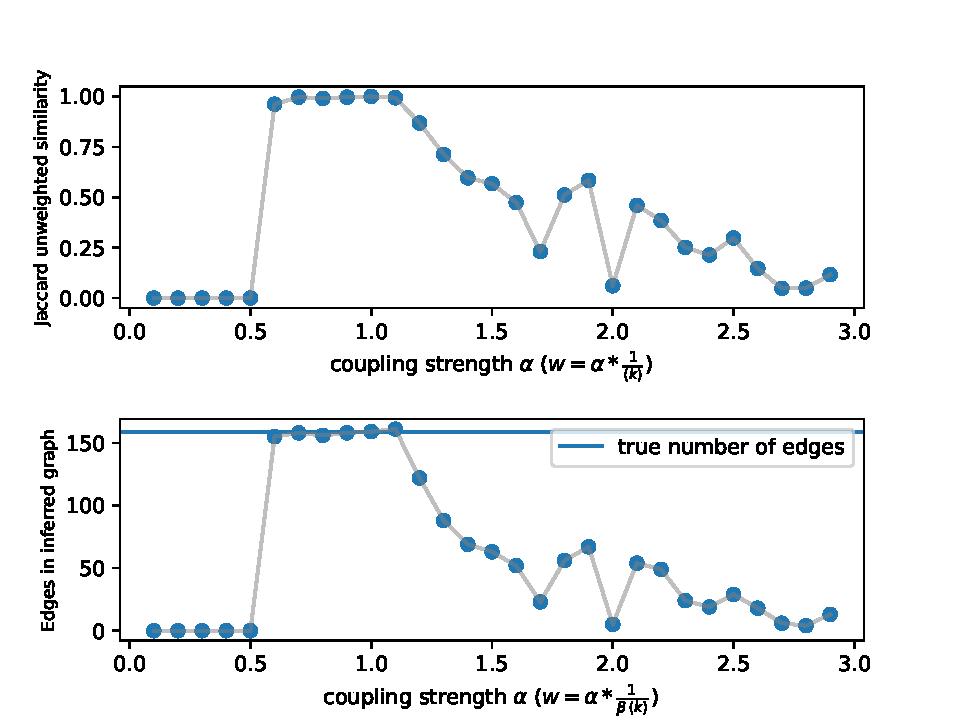
\includegraphics[width=\linewidth]{images/coupling.pdf}
    \caption{}
    \label{fig:enter-label}
\end{figure}
Come si vede dal grafico, per couplings troppo deboli (fase disordinata) l'inferenza fallisce, poi a partire da $\alpha \simeq 0.5$ (suppongo valore critico) è molto buona, per poi degradare lentamente.
Il valore critico secondo formula mia doveva essere $\alpha = 1$ ma probabilmente c'è un fattore due di differenza nella definizione dell'hamiltoniana. Not a big deal.

\textbf{Tempo di simulazione} 30 minuti.

\section{Dipendenza dal numero di samples M}
Bene, adesso che abbiamo verificato che se la dinamica di Ising si discosta troppo dal regime critico l'algoritmo di inferenza non funziona più, andiamo a vedere come si comporta invece nella zona di massima performance se invece cambiamo il numero di sample $M$ usati per l'inferenza e il numero di nodi $N$ del grafo.
Nel seguito la weight matrix del network sarà sempre definita come 
\begin{equation}
    W_{i,\,j} =
    \begin{cases}
         \frac{1}{\langle k \rangle} \quad se \quad i\longleftrightarrow j \\
    0 \quad altrimenti
    \end{cases}
\end{equation}
Usiamo lo stesso piccolo network della sezione precedente, con $62$ nodi. 
\begin{figure}[H]
    \centering
    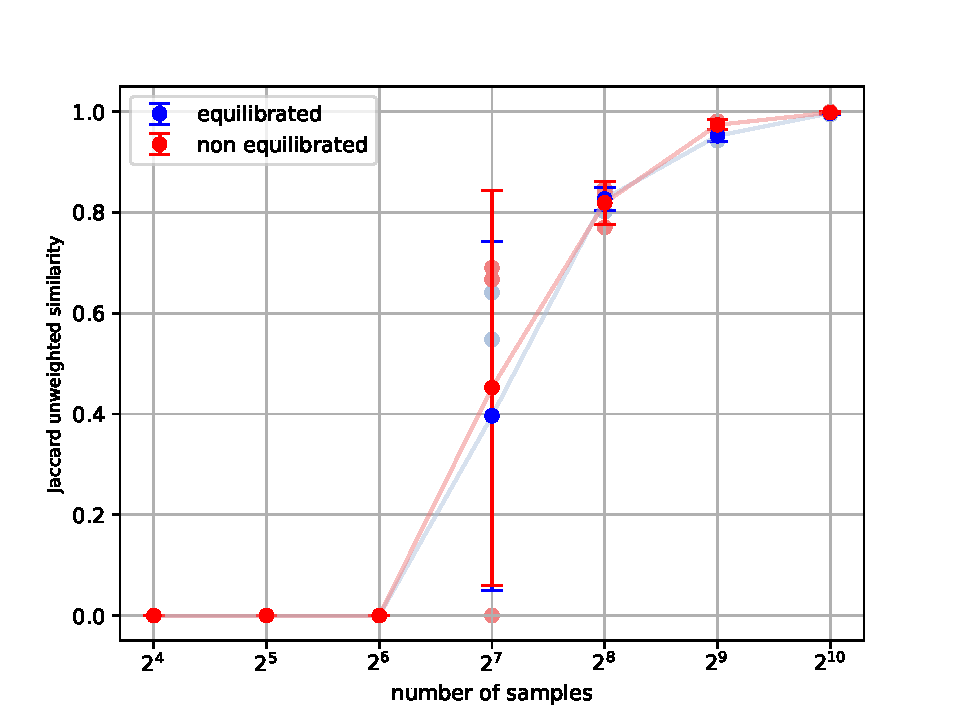
\includegraphics[width=\linewidth]{images/sampling.pdf}
    \caption{Ricostruzione con \textbf{IsingGlauberBlockState()} (modello dinamico).
     Dati mediati su $3$ realizzazioni indipendenti della dinamica di Glauber su modello di Ising. Ogni realizzazione conteneva $1024$ samples. Per la ricostruzione si sono presi gli ultimi $m$ samples (es: $m = 128$, samples da $1024-128$ a $1024$) per assicurare che il sistema fosse equilibrato (rosso)  oppure i sample sono presi all'inizio della dinamica (non equilibrato, blu). Non c'è differenza, vuol dire che il modello dinamico di inferenza funziona come deve. Dentro la libreria c'è anche la versione statica dell'algoritmo di inferenza, si chiama \textbf{PseudoIsingBlockState()} e funziona solo se i sample sono presi all'equilibrio.}
    \label{fig:enter-label}
\end{figure}


\section{Dipendenza dal numero di nodi N e di samples M}
In questa sezione i risultati dell'analisi di come scala l'accuratezza della ricostruzione con il numero di nodi $N$ del grafo e il numero di samples $M$ utilizzati per l'inferenza. I grafi sono realizzazioni di Stochastic Block Models con numero di nodi $[64, 128, 256, 512]$, grado medio $k = 4$, probabilità fissa di connessioni intra e inter- gruppo, numero di partizioni $= N^{\frac{1}{3}}$. La dinamica di Ising è stata simulata una sola volta su ogni grafo, poi l'inferenza su quella dinamica è stata ripetuta più volte variando il numero di samples del campione. L'accuratezza è misurata con il coefficiente di Jaccard.

\begin{figure}[H]
    \centering
    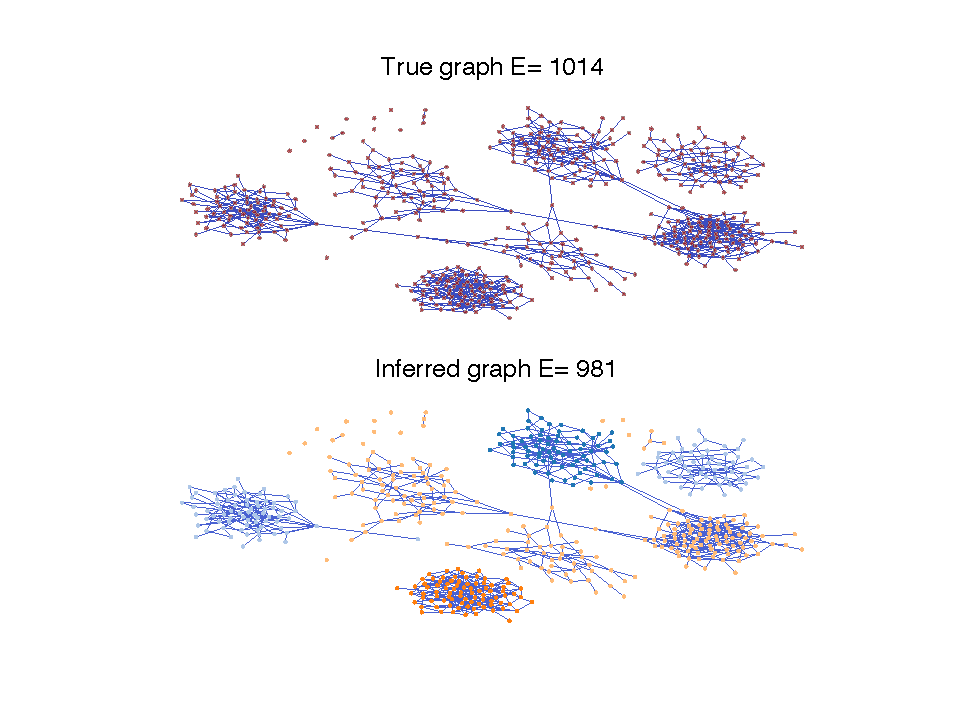
\includegraphics[width=\linewidth]{images/visualization.pdf}
    \caption{Esempio di risultato di inferenza su uno stochastic block model con $N = 512$ e $M = 900$ samples usati per l'inferenza. L'inferenza è molto accurata, con indici di Jaccard $J(A, \Tilde{A}) =0.97$, $J(A, \Tilde{A}): 0.92$. Le comunità inferite corrispondono a quelle reali.}
\end{figure}.
\begin{figure}[H]
    \centering
    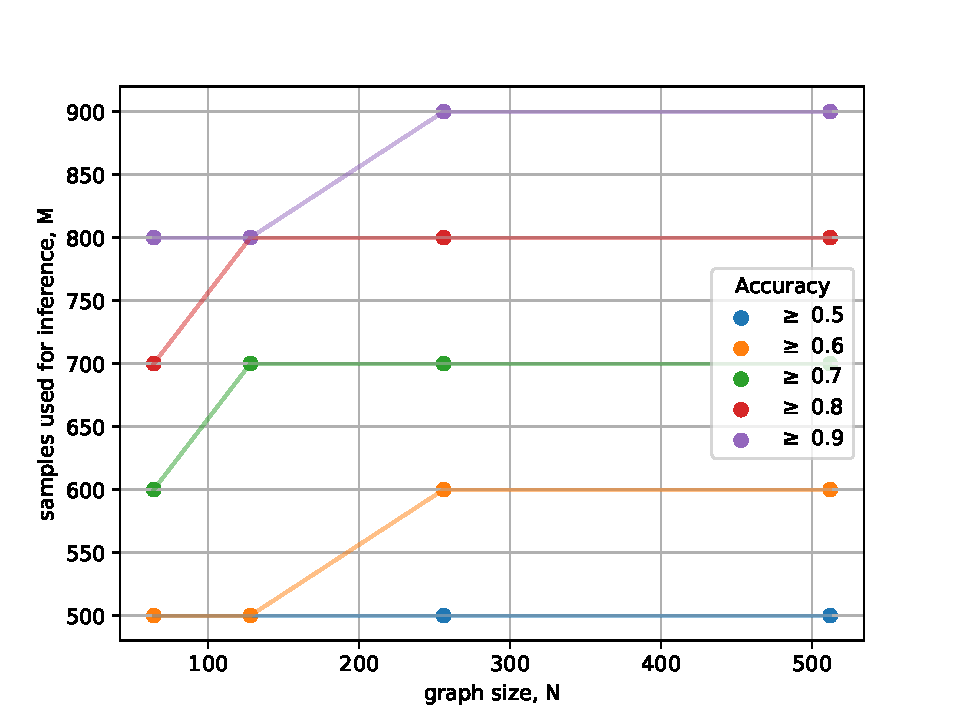
\includegraphics[width=0.45\linewidth]{images/plain_sbm_ising.pdf}
    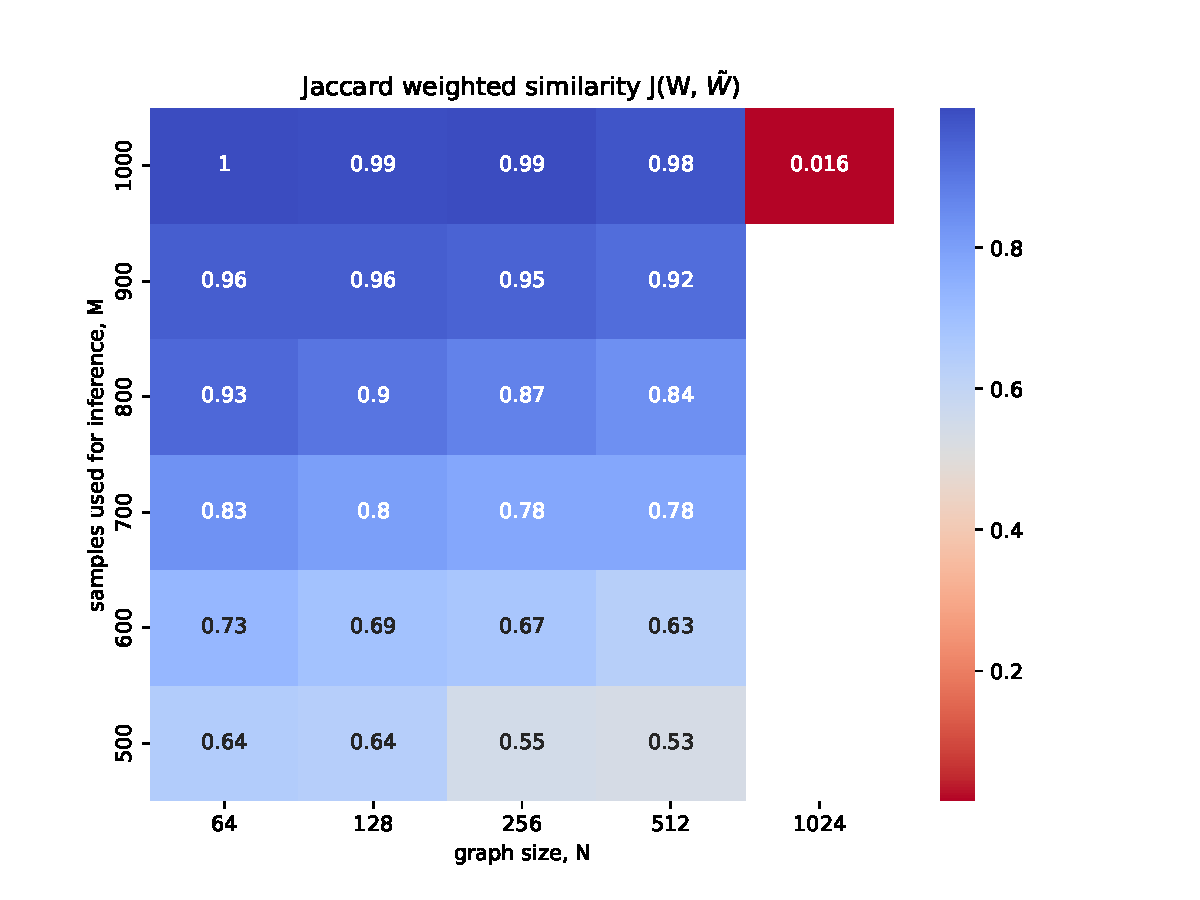
\includegraphics[width=0.45\linewidth]{images/sbm_ising_heatmap.pdf}
    \caption{Risultati aggregati. Ogni punto si riferisce ad un solo grafo, (non ho mediato diverse realizzazioni per motivi di tempo). Manca l'informazione sul tempo di esecuzione (me ne sono dimenticata!) ma indicativamente è nell'ordine di  $\simeq 20$ minuti per il grafo da $512$ nodi. \textbf{Parametro beta fissato come $beta = 1$ (!! diverso da 1/k medio)}}
    \label{fig:enter-label}
\end{figure}

\section{Accuracy of inference with respect to number of samples}
\subsection{Setup}
The algorithm is tested using input time series data from a simulated Ising-Glauber dynamics.
    The graphs used in this test are synthetic, undirected, and free of self-loops and multi-edges.
    They are generated from a stochastic block model (SBM) with N nodes and approximately  $N^{\frac{1}{3}}$  partitions.
    The probability of intra-partition connections is set to $0.999$, while the probability of inter-partition connections is set to $0.001$. This structure results in partitions that are highly likely to form disjoint connected components. The mean degree is set to $k_mean = 4$. The Ising dynamics is simulated for a fixed value of the inverse temperature $beta = 1$. The graphs are given uniform weights = $1/ k_mean$. This combination of weights and inverse temperature results in a partially ordered regime for the Ising dynamics, thus enabling inference.
\subsection{Results}
\begin{figure}[H]
    \centering
    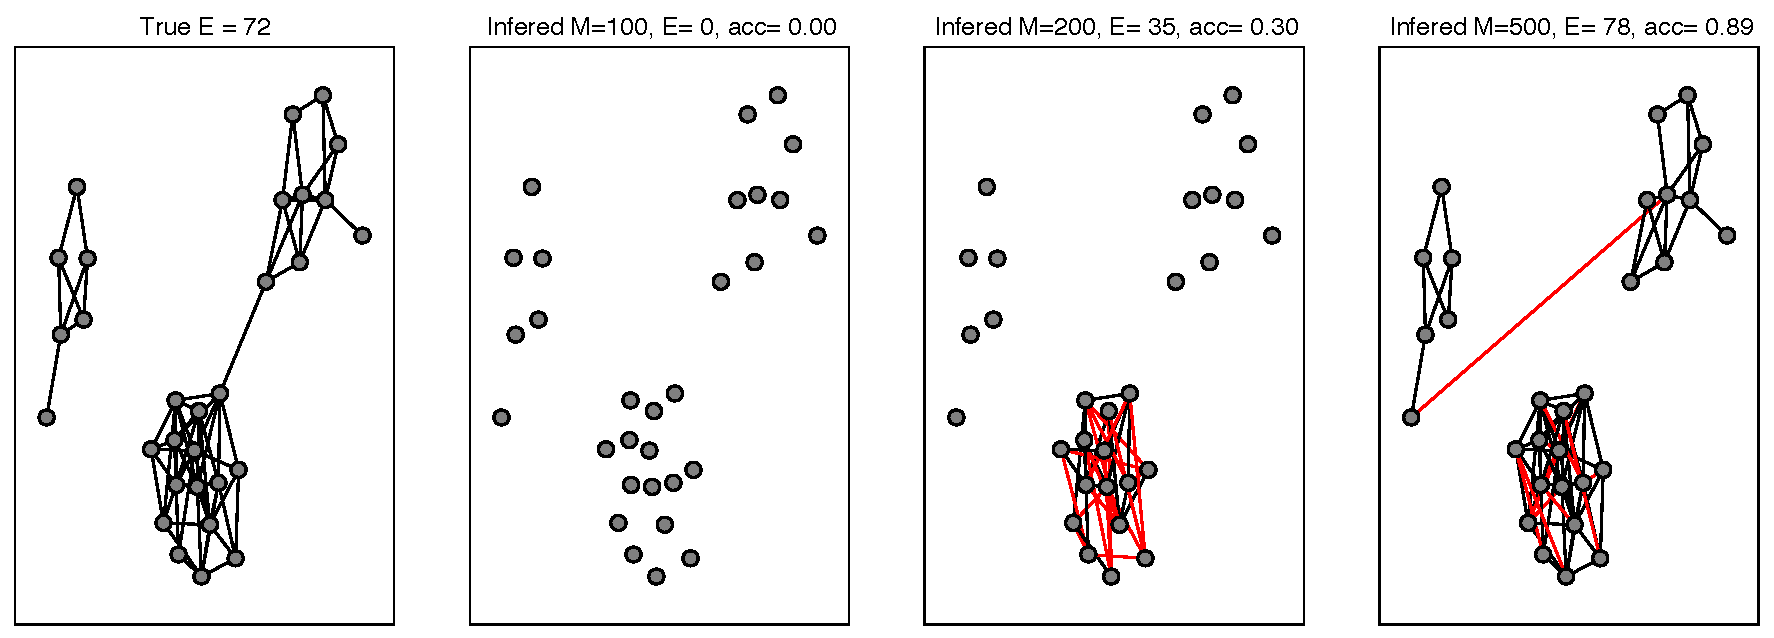
\includegraphics[width=\linewidth]{images/sample_visualization_30_nodes.pdf}
    \caption{A sample visualization of the accuracy of the inference with varying number of samples, for a graph with $N = 30, E=72$. Spurious edges (infered edges that are not present in the true graph) are coloured red. The accuracy coefficient refers to the Jaccard unweighted similarity.}
    \label{fig:sample_visualization}
\end{figure}
In principle, many factors may vary the quality of the reconstruction from dynamics, the most obvious is the number of samples used, $M$ in all the following. However, in principle graphs with different topology might need a different number of samples in order for inference to achieve the same accuracy. Another problem that arises when dealing with experimental data like our mice data is that often successive samples are not separed by the same time length (e.g. first sample taken on day one, second sample taken on day five and third sample taken on day eleven...). For this reason it is worthy to check on simulated data at least how much the accuracy of inference deteriorates when samples are not consecutive in time with respect to when they are. The following plot \ref{fig:consecutive_times} shows results on a sample of $40$ graphs generated as said in the setup. Another thing that one can see from the plot is that there is a bimodal trend: for some fixed node number, there are graphs for which the inference fails completely (jaccard $=0$, meaning the infered graph is the null graph) and other where it works. This effect should disappear with increasing number of samples, where ideally inference is expected to work independently of the particular graph instance.

\begin{figure}[H]
    \centering
    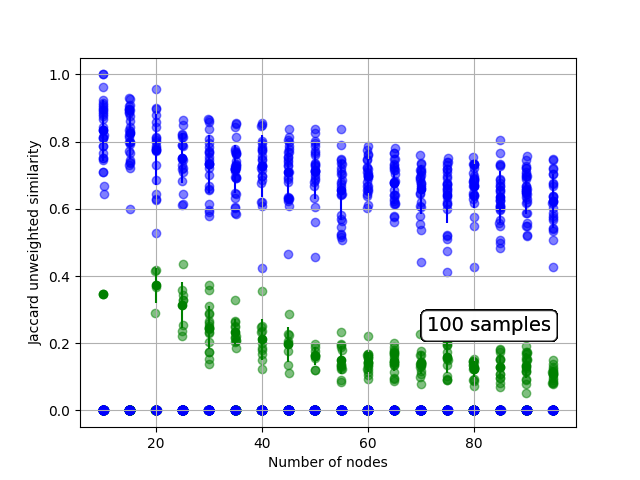
\includegraphics[width=0.9\linewidth]{images/jaccard_vs_nodes_100_samples.png}
    \caption{Jaccard unweighted accuracy versus the number of nodes in the graph. Blue color correspond to the case where inference was made from a set of $M= 100$ consecutive samples, green when samples where chosen at random inside the timeseries, but still ordered chronologically. One can see that the quality of inference significately decreases when samples are chosen with random intervals inbetween them. The experimental data is something in between the two extremes: the interval between consecutive measures is not fixed but it is not too broadly distributed around some value.}
    \label{fig:enter-label}
\end{figure}
\begin{figure}[H]
    \centering
    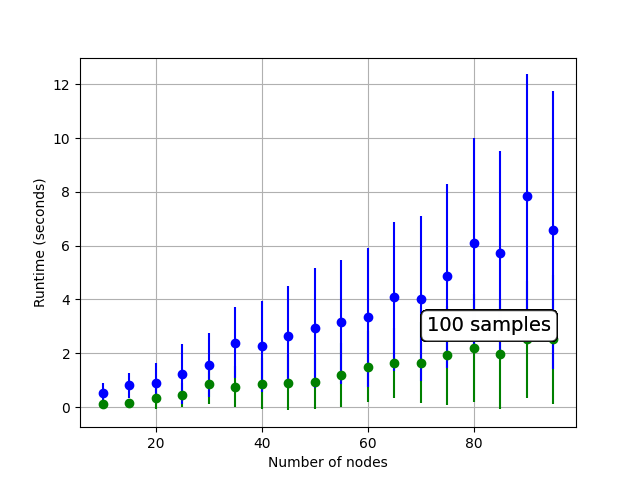
\includegraphics[width=0.5\linewidth]{images/runtime_vs_nodes_100_samples.png}
    \caption{Mean runtime of the inference algorithm. In blue when samples have fixed in-between intervals, in green when not.}
    \label{fig:enter-label}
\end{figure}
\subsection{Inferenza con modello dinamico IsingGlauberBlockState}
Analisi propedeutica all'utilizzo del modello di Ising sui dati di microbioma presenza/assenza.
I dati si riferiscono ad una sola istanza di grafo per ciascuna dimensione fissata $N$. La dinamica è simulata una sola volta su ciascun grafo. L'inferenza è stata eseguite una sola volta sulla dinamica. Per migliorare la precisione del test bisognerebbe aumentare il campione di grafi e fare l'inferenza più volte sullo stesso grafo.
\textbf{Parametro beta fissato come $beta = 1$ (!! diverso da 1/k medio)}.
Invece mettendo $beta = 1/k medio$ non funziona l'inferenza. Controlla perchè.

Sui topi abbiamo $100- 200$ sample per topo. Da queste simulazioni, con tale numero di sample appare altamente improbabile riuscire a fare inferenza assumendo un modello di Ising. L'accuratezza è all'incirca nel range $[0.3 - 0.5]$ su dinamiche davvero di Ising.
\begin{figure}[H]
    \centering
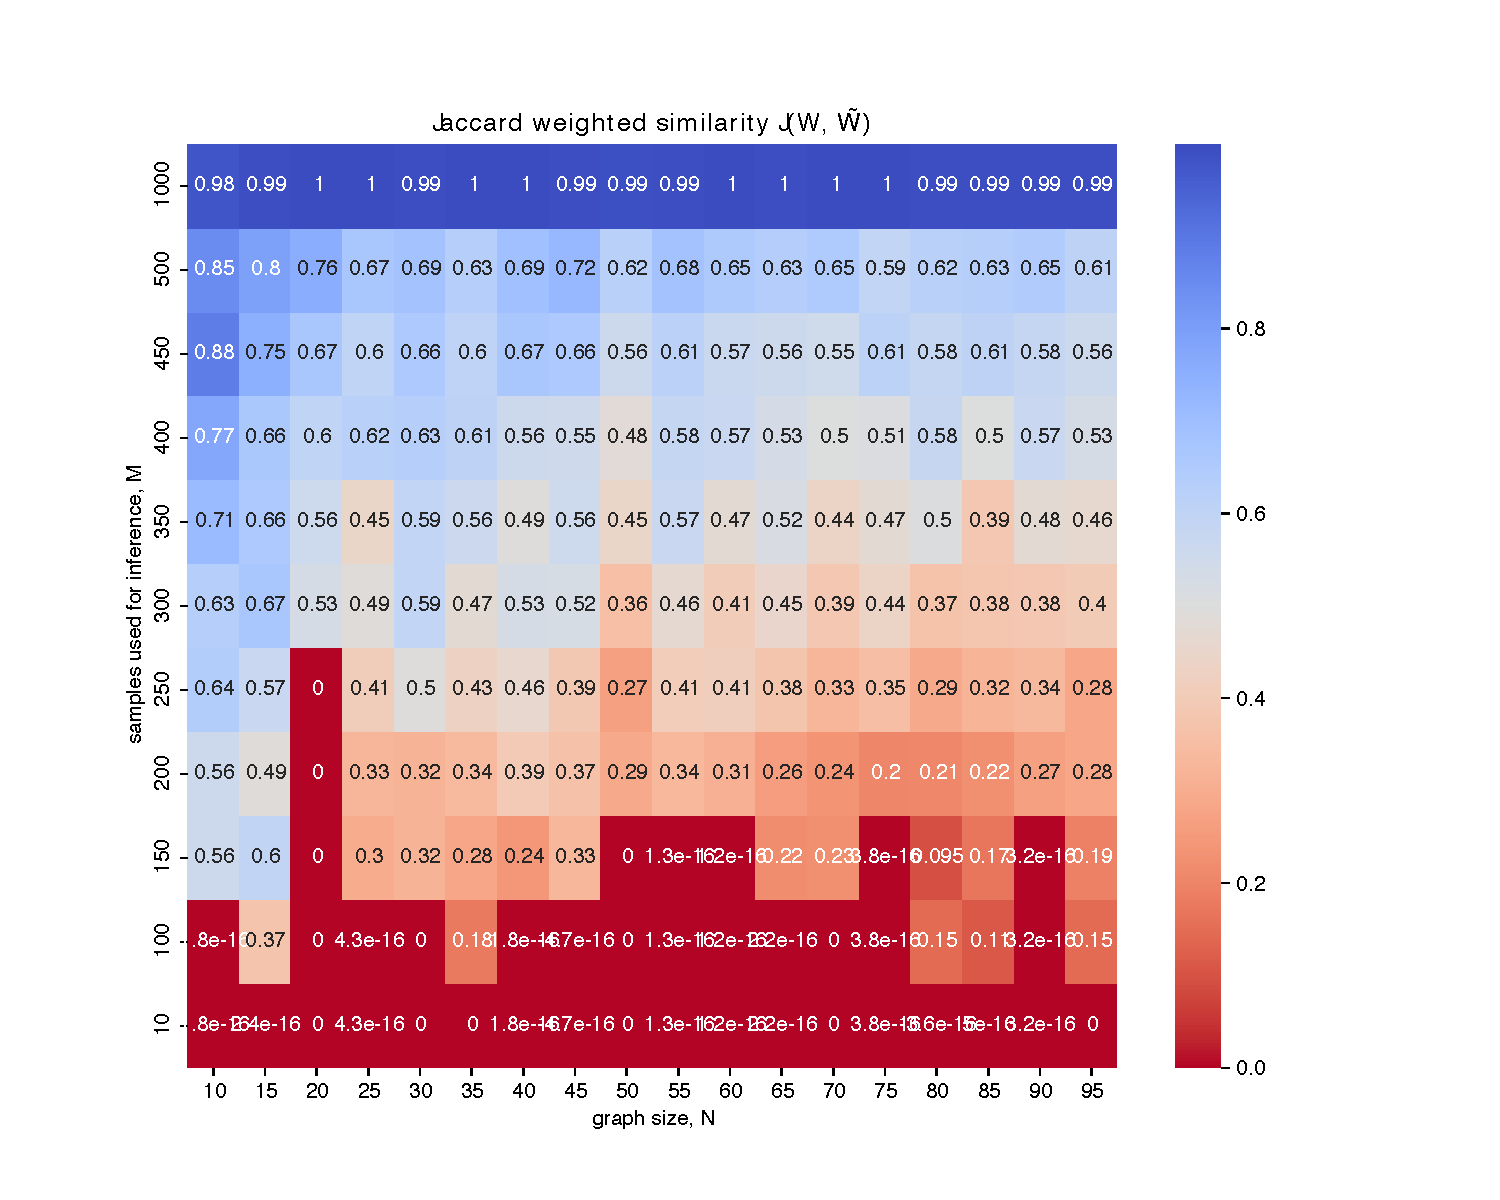
\includegraphics[width=0.8\linewidth]{images/sbm_ising_heatmap_small.pdf}
    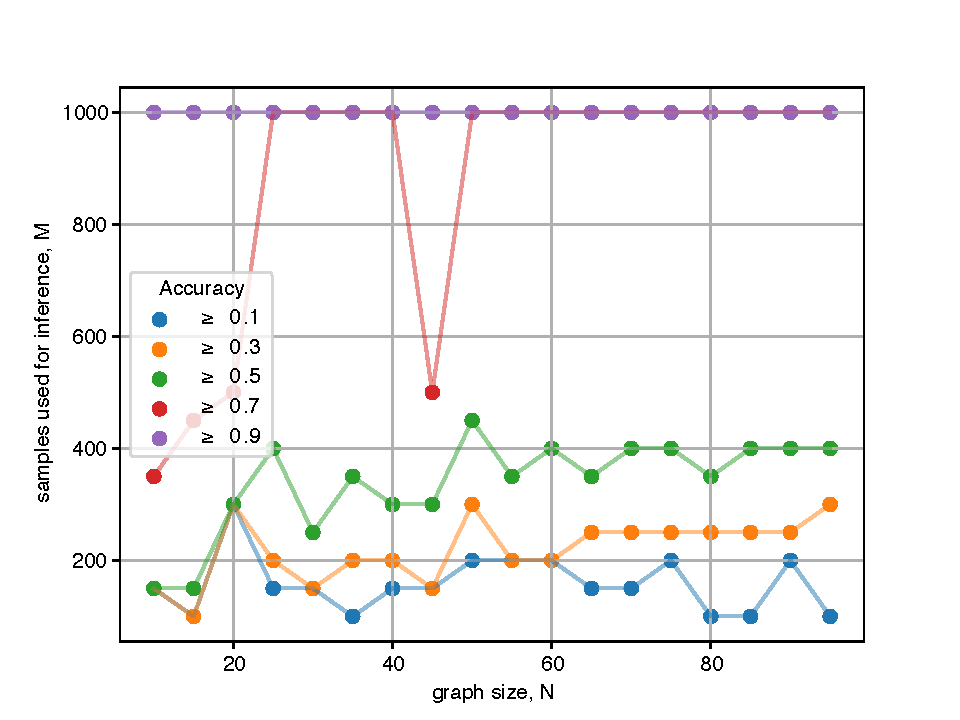
\includegraphics[width=0.6\linewidth]{images/sbm_ising_contour_small.pdf}
    \caption{}
\end{figure}


\subsection{Inferenza con modello statico (equilibrio)}


\end{document}
